
\subsection*{task 1.6 \\[1ex] getting used to meshgrids (part 1)}

Read image \texttt{portrait.png} into an array \texttt{arrF}. Then ---without using \keyword{for} loops--- set the intensities of all its pixels situated within an ellipse of width $2 \cdot 50$ and height $2 \cdot 85$ which is centered at array coordinates $\bigl[ c_i, c_j \bigr] = \bigl[ 128, 110 \bigr]$ to $255$. Write your result as a PNG image. \\[1ex]
%%%%%
%%%%%
%%%%% enter your code into the following environment
%%%%%
%%%%%
\begin{python}
# paste your code here

\end{python}
%%%%%
%%%%%
%%%%%
%%%%%
%%%%%



\vspace{1cm}
To illustrate how your resulting image should look like, here is the result you would obtain from working with width $2 \cdot 100$, height $2 \cdot 50$ and center point $\bigl[ 128, 128 \bigr]$
%%%%%
%%%%%
%%%%% enter your result here, i.e. replace "t1-6.png" by the name of your resulting image file
%%%%%
%%%%%
\begin{center}
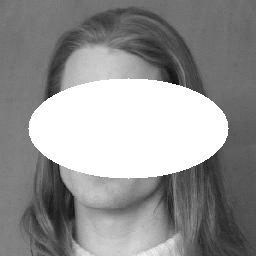
\includegraphics[width=0.5\textwidth]{t1-6.png} 
\end{center}
%%%%%
%%%%%
%%%%%
%%%%%
%%%%%
Simply replace the above image with the image you just created.






